\documentclass[1p]{elsarticle_modified}
%\bibliographystyle{elsarticle-num}

%\usepackage[colorlinks]{hyperref}
%\usepackage{abbrmath_seonhwa} %\Abb, \Ascr, \Acal ,\Abf, \Afrak
\usepackage{amsfonts}
\usepackage{amssymb}
\usepackage{amsmath}
\usepackage{amsthm}
\usepackage{scalefnt}
\usepackage{amsbsy}
\usepackage{kotex}
\usepackage{caption}
\usepackage{subfig}
\usepackage{color}
\usepackage{graphicx}
\usepackage{xcolor} %% white, black, red, green, blue, cyan, magenta, yellow
\usepackage{float}
\usepackage{setspace}
\usepackage{hyperref}

\usepackage{tikz}
\usetikzlibrary{arrows}

\usepackage{multirow}
\usepackage{array} % fixed length table
\usepackage{hhline}

%%%%%%%%%%%%%%%%%%%%%
\makeatletter
\renewcommand*\env@matrix[1][\arraystretch]{%
	\edef\arraystretch{#1}%
	\hskip -\arraycolsep
	\let\@ifnextchar\new@ifnextchar
	\array{*\c@MaxMatrixCols c}}
\makeatother %https://tex.stackexchange.com/questions/14071/how-can-i-increase-the-line-spacing-in-a-matrix
%%%%%%%%%%%%%%%

\usepackage[normalem]{ulem}

\newcommand{\msout}[1]{\ifmmode\text{\sout{\ensuremath{#1}}}\else\sout{#1}\fi}
%SOURCE: \msout is \stkout macro in https://tex.stackexchange.com/questions/20609/strikeout-in-math-mode

\newcommand{\cancel}[1]{
	\ifmmode
	{\color{red}\msout{#1}}
	\else
	{\color{red}\sout{#1}}
	\fi
}

\newcommand{\add}[1]{
	{\color{blue}\uwave{#1}}
}

\newcommand{\replace}[2]{
	\ifmmode
	{\color{red}\msout{#1}}{\color{blue}\uwave{#2}}
	\else
	{\color{red}\sout{#1}}{\color{blue}\uwave{#2}}
	\fi
}

\newcommand{\Sol}{\mathcal{S}} %segment
\newcommand{\D}{D} %diagram
\newcommand{\A}{\mathcal{A}} %arc


%%%%%%%%%%%%%%%%%%%%%%%%%%%%%5 test

\def\sl{\operatorname{\textup{SL}}(2,\Cbb)}
\def\psl{\operatorname{\textup{PSL}}(2,\Cbb)}
\def\quan{\mkern 1mu \triangleright \mkern 1mu}

\theoremstyle{definition}
\newtheorem{thm}{Theorem}[section]
\newtheorem{prop}[thm]{Proposition}
\newtheorem{lem}[thm]{Lemma}
\newtheorem{ques}[thm]{Question}
\newtheorem{cor}[thm]{Corollary}
\newtheorem{defn}[thm]{Definition}
\newtheorem{exam}[thm]{Example}
\newtheorem{rmk}[thm]{Remark}
\newtheorem{alg}[thm]{Algorithm}

\newcommand{\I}{\sqrt{-1}}
\begin{document}

%\begin{frontmatter}
%
%\title{Boundary parabolic representations of knots up to 8 crossings}
%
%%% Group authors per affiliation:
%\author{Yunhi Cho} 
%\address{Department of Mathematics, University of Seoul, Seoul, Korea}
%\ead{yhcho@uos.ac.kr}
%
%
%\author{Seonhwa Kim} %\fnref{s_kim}}
%\address{Center for Geometry and Physics, Institute for Basic Science, Pohang, 37673, Korea}
%\ead{ryeona17@ibs.re.kr}
%
%\author{Hyuk Kim}
%\address{Department of Mathematical Sciences, Seoul National University, Seoul 08826, Korea}
%\ead{hyukkim@snu.ac.kr}
%
%\author{Seokbeom Yoon}
%\address{Department of Mathematical Sciences, Seoul National University, Seoul, 08826,  Korea}
%\ead{sbyoon15@snu.ac.kr}
%
%\begin{abstract}
%We find all boundary parabolic representation of knots up to 8 crossings.
%
%\end{abstract}
%\begin{keyword}
%    \MSC[2010] 57M25 
%\end{keyword}
%
%\end{frontmatter}

%\linenumbers
%\tableofcontents
%
\newcommand\colored[1]{\textcolor{white}{\rule[-0.35ex]{0.8em}{1.4ex}}\kern-0.8em\color{red} #1}%
%\newcommand\colored[1]{\textcolor{white}{ #1}\kern-2.17ex	\textcolor{white}{ #1}\kern-1.81ex	\textcolor{white}{ #1}\kern-2.15ex\color{red}#1	}

{\Large $\underline{12a_{0244}~(K12a_{0244})}$}

\setlength{\tabcolsep}{10pt}
\renewcommand{\arraystretch}{1.6}
\vspace{1cm}\begin{tabular}{m{100pt}>{\centering\arraybackslash}m{274pt}}
\multirow{5}{120pt}{
	\centering
	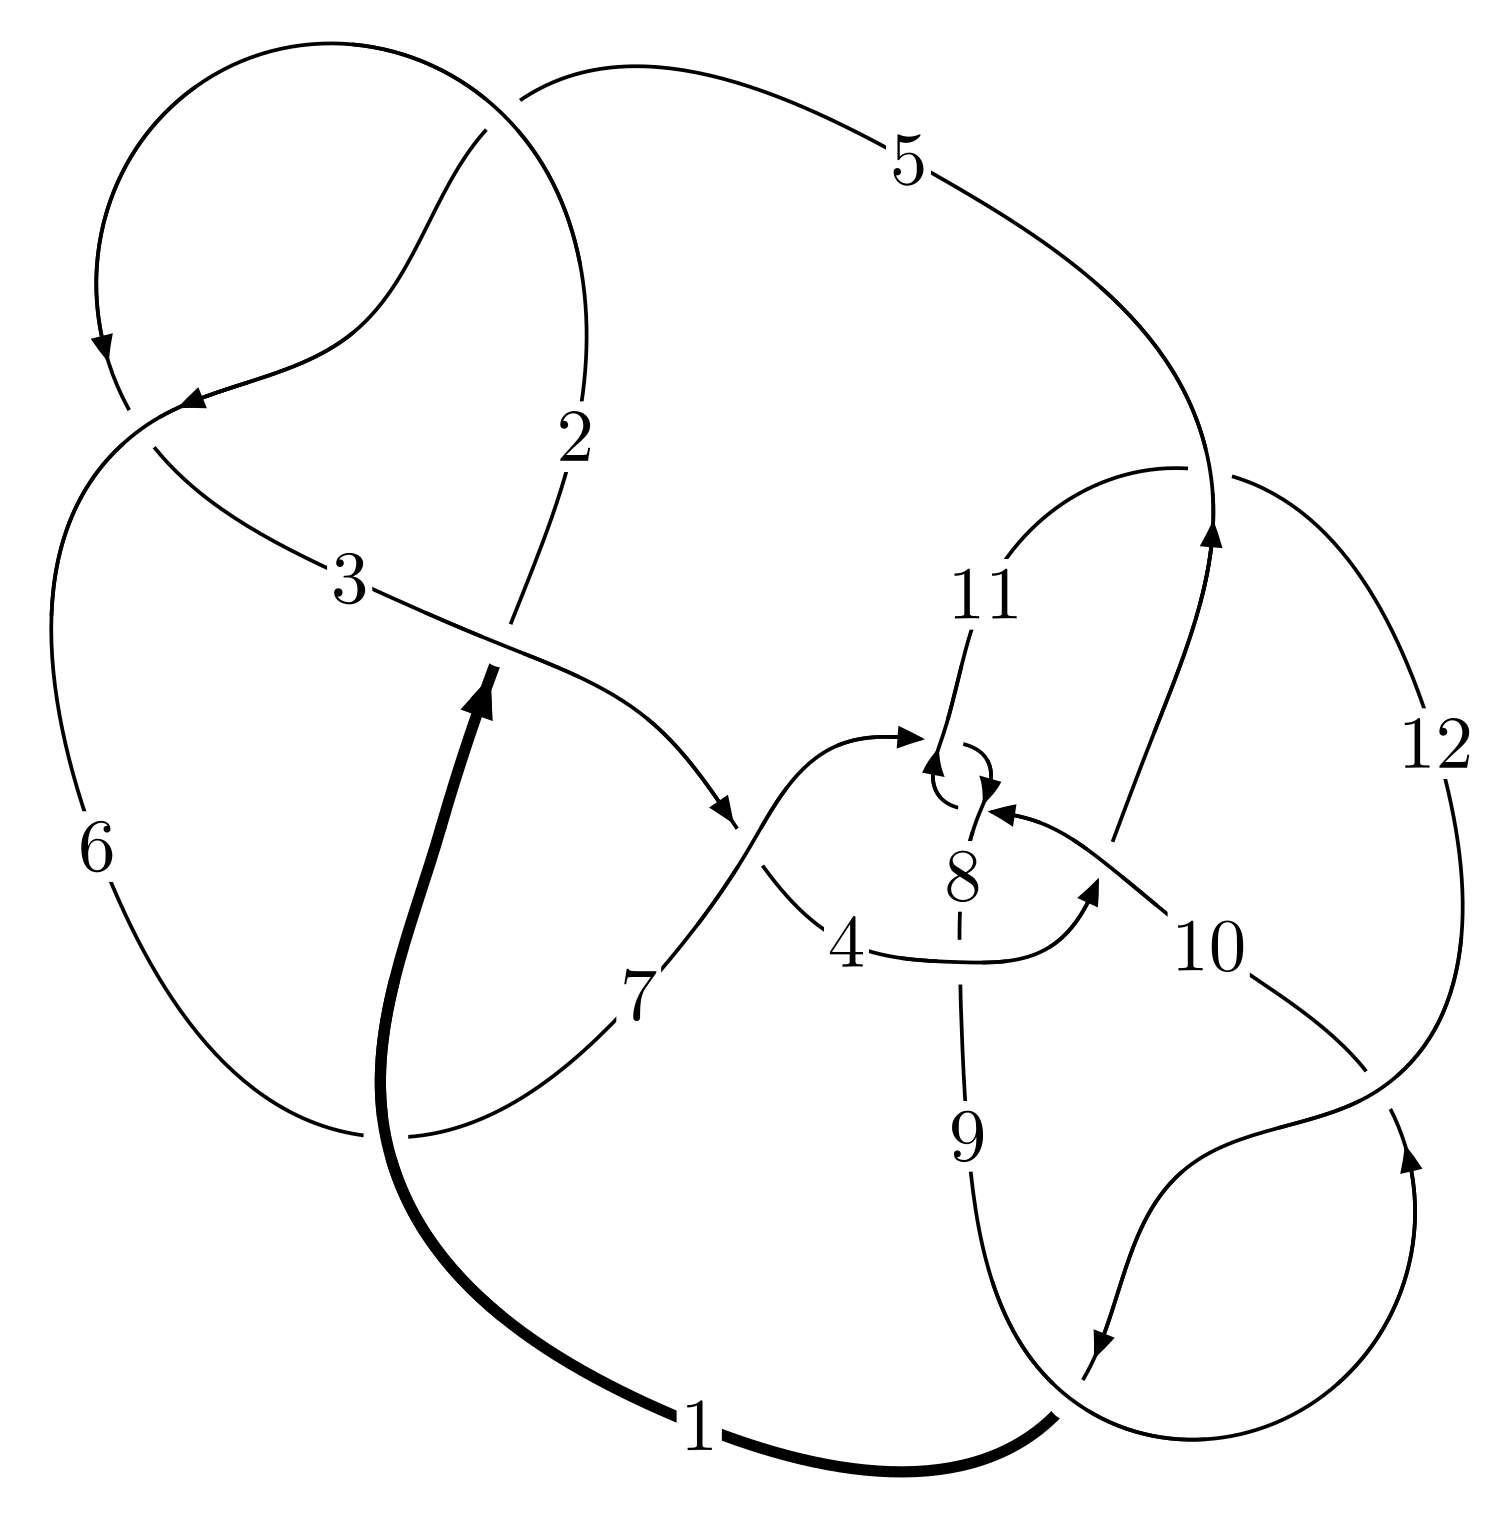
\includegraphics[width=112pt]{../../../GIT/diagram.site/Diagrams/png/1045_12a_0244.png}\\
\ \ \ A knot diagram\footnotemark}&
\allowdisplaybreaks
\textbf{Linearized knot diagam} \\
\cline{2-2}
 &
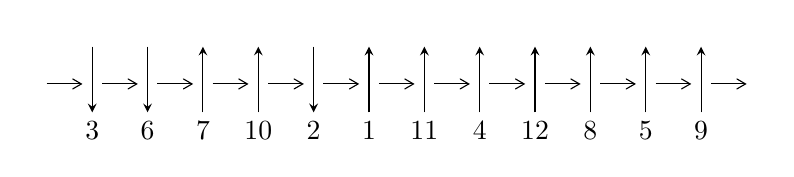
\begin{tikzpicture}[x=20pt, y=17pt]
	% nodes
	\node (C0) at (0, 0) {};
	\node (C1) at (1, 0) {};
	\node (C1U) at (1, +1) {};
	\node (C1D) at (1, -1) {3};

	\node (C2) at (2, 0) {};
	\node (C2U) at (2, +1) {};
	\node (C2D) at (2, -1) {6};

	\node (C3) at (3, 0) {};
	\node (C3U) at (3, +1) {};
	\node (C3D) at (3, -1) {7};

	\node (C4) at (4, 0) {};
	\node (C4U) at (4, +1) {};
	\node (C4D) at (4, -1) {10};

	\node (C5) at (5, 0) {};
	\node (C5U) at (5, +1) {};
	\node (C5D) at (5, -1) {2};

	\node (C6) at (6, 0) {};
	\node (C6U) at (6, +1) {};
	\node (C6D) at (6, -1) {1};

	\node (C7) at (7, 0) {};
	\node (C7U) at (7, +1) {};
	\node (C7D) at (7, -1) {11};

	\node (C8) at (8, 0) {};
	\node (C8U) at (8, +1) {};
	\node (C8D) at (8, -1) {4};

	\node (C9) at (9, 0) {};
	\node (C9U) at (9, +1) {};
	\node (C9D) at (9, -1) {12};

	\node (C10) at (10, 0) {};
	\node (C10U) at (10, +1) {};
	\node (C10D) at (10, -1) {8};

	\node (C11) at (11, 0) {};
	\node (C11U) at (11, +1) {};
	\node (C11D) at (11, -1) {5};

	\node (C12) at (12, 0) {};
	\node (C12U) at (12, +1) {};
	\node (C12D) at (12, -1) {9};
	\node (C13) at (13, 0) {};

	% arrows
	\draw[->,>={angle 60}]
	(C0) edge (C1) (C1) edge (C2) (C2) edge (C3) (C3) edge (C4) (C4) edge (C5) (C5) edge (C6) (C6) edge (C7) (C7) edge (C8) (C8) edge (C9) (C9) edge (C10) (C10) edge (C11) (C11) edge (C12) (C12) edge (C13) ;	\draw[->,>=stealth]
	(C1U) edge (C1D) (C2U) edge (C2D) (C3D) edge (C3U) (C4D) edge (C4U) (C5U) edge (C5D) (C6D) edge (C6U) (C7D) edge (C7U) (C8D) edge (C8U) (C9D) edge (C9U) (C10D) edge (C10U) (C11D) edge (C11U) (C12D) edge (C12U) ;
	\end{tikzpicture} \\
\hhline{~~} \\& 
\textbf{Solving Sequence} \\ \cline{2-2} 
 &
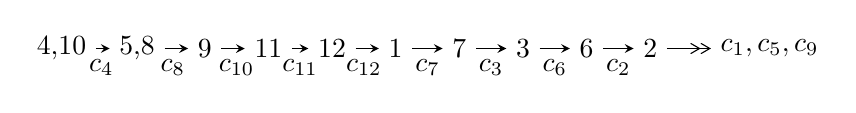
\begin{tikzpicture}[x=23pt, y=7pt]
	% node
	\node (A0) at (-1/8, 0) {4,10};
	\node (A1) at (17/16, 0) {5,8};
	\node (A2) at (17/8, 0) {9};
	\node (A3) at (25/8, 0) {11};
	\node (A4) at (33/8, 0) {12};
	\node (A5) at (41/8, 0) {1};
	\node (A6) at (49/8, 0) {7};
	\node (A7) at (57/8, 0) {3};
	\node (A8) at (65/8, 0) {6};
	\node (A9) at (73/8, 0) {2};
	\node (C1) at (1/2, -1) {$c_{4}$};
	\node (C2) at (13/8, -1) {$c_{8}$};
	\node (C3) at (21/8, -1) {$c_{10}$};
	\node (C4) at (29/8, -1) {$c_{11}$};
	\node (C5) at (37/8, -1) {$c_{12}$};
	\node (C6) at (45/8, -1) {$c_{7}$};
	\node (C7) at (53/8, -1) {$c_{3}$};
	\node (C8) at (61/8, -1) {$c_{6}$};
	\node (C9) at (69/8, -1) {$c_{2}$};
	\node (A10) at (11, 0) {$c_{1},c_{5},c_{9}$};

	% edge
	\draw[->,>=stealth]	
	(A0) edge (A1) (A1) edge (A2) (A2) edge (A3) (A3) edge (A4) (A4) edge (A5) (A5) edge (A6) (A6) edge (A7) (A7) edge (A8) (A8) edge (A9) ;
	\draw[->>,>={angle 60}]	
	(A9) edge (A10);
\end{tikzpicture} \\ 

\end{tabular} \\

\footnotetext{
The image of knot diagram is generated by the software ``\textbf{Draw programme}" developed by Andrew Bartholomew(\url{http://www.layer8.co.uk/maths/draw/index.htm\#Running-draw}), where we modified some parts for our purpose(\url{https://github.com/CATsTAILs/LinksPainter}).
}\phantom \\ \newline 
\centering \textbf{Ideals for irreducible components\footnotemark of $X_{\text{par}}$} 
 
\begin{align*}
I^u_{1}&=\langle 
-2.70055\times10^{176} u^{48}+7.34394\times10^{176} u^{47}+\cdots+3.67864\times10^{181} b+1.37942\times10^{180},\\
\phantom{I^u_{1}}&\phantom{= \langle  }1.66691\times10^{178} u^{48}-4.46314\times10^{178} u^{47}+\cdots+7.35728\times10^{181} a-1.26886\times10^{182},\\
\phantom{I^u_{1}}&\phantom{= \langle  }u^{49}-3 u^{48}+\cdots+22528 u-8192\rangle \\
I^u_{2}&=\langle 
u^{39}+u^{38}+\cdots+b+a,\;- u^{38}- u^{37}+\cdots+a^2-2 u,\;u^{40}+u^{39}+\cdots+2 u^3+1\rangle \\
I^u_{3}&=\langle 
b+u-1,\;a+1,\;u^2+1\rangle \\
\\
I^v_{1}&=\langle 
a,\;v^5-2 v^4+16 v^2+64 b-16 v-32,\;v^6-2 v^5+16 v^3-16 v^2-32 v+64\rangle \\
\end{align*}
\raggedright * 4 irreducible components of $\dim_{\mathbb{C}}=0$, with total 137 representations.\\
\footnotetext{All coefficients of polynomials are rational numbers. But the coefficients are sometimes approximated in decimal forms when there is not enough margin.}
\newpage
\renewcommand{\arraystretch}{1}
\centering \section*{I. $I^u_{1}= \langle -2.70\times10^{176} u^{48}+7.34\times10^{176} u^{47}+\cdots+3.68\times10^{181} b+1.38\times10^{180},\;1.67\times10^{178} u^{48}-4.46\times10^{178} u^{47}+\cdots+7.36\times10^{181} a-1.27\times10^{182},\;u^{49}-3 u^{48}+\cdots+22528 u-8192 \rangle$}
\flushleft \textbf{(i) Arc colorings}\\
\begin{tabular}{m{7pt} m{180pt} m{7pt} m{180pt} }
\flushright $a_{4}=$&$\begin{pmatrix}1\\0\end{pmatrix}$ \\
\flushright $a_{10}=$&$\begin{pmatrix}0\\u\end{pmatrix}$ \\
\flushright $a_{5}=$&$\begin{pmatrix}1\\- u^2\end{pmatrix}$ \\
\flushright $a_{8}=$&$\begin{pmatrix}-0.000226567 u^{48}+0.000606629 u^{47}+\cdots+1.52293 u+1.72464\\7.34115\times10^{-6} u^{48}-0.0000199637 u^{47}+\cdots+0.829123 u-0.0374982\end{pmatrix}$ \\
\flushright $a_{9}=$&$\begin{pmatrix}-0.000219225 u^{48}+0.000586666 u^{47}+\cdots+2.35206 u+1.68714\\7.34115\times10^{-6} u^{48}-0.0000199637 u^{47}+\cdots+0.829123 u-0.0374982\end{pmatrix}$ \\
\flushright $a_{11}=$&$\begin{pmatrix}0.000219225 u^{48}-0.000586666 u^{47}+\cdots-2.35206 u-1.68714\\0.0000401811 u^{48}-0.000116259 u^{47}+\cdots+0.632956 u-0.619217\end{pmatrix}$ \\
\flushright $a_{12}=$&$\begin{pmatrix}0.000226567 u^{48}-0.000606629 u^{47}+\cdots-1.52293 u-1.72464\\0.0000425308 u^{48}-0.000121702 u^{47}+\cdots+0.619218 u-0.636090\end{pmatrix}$ \\
\flushright $a_{1}=$&$\begin{pmatrix}0.000485973 u^{48}-0.00130955 u^{47}+\cdots-4.24203 u-4.03099\\0.0000827120 u^{48}-0.000237961 u^{47}+\cdots+0.252174 u-1.25531\end{pmatrix}$ \\
\flushright $a_{7}=$&$\begin{pmatrix}-0.000485973 u^{48}+0.00130955 u^{47}+\cdots+4.24203 u+4.03099\\8.34395\times10^{-6} u^{48}-0.0000219487 u^{47}+\cdots+0.890893 u-0.0398997\end{pmatrix}$ \\
\flushright $a_{3}=$&$\begin{pmatrix}-0.000168254 u^{48}+0.000608654 u^{47}+\cdots+21.4016 u-4.40654\\-0.0000103751 u^{48}+0.0000252373 u^{47}+\cdots-0.598442 u+0.217313\end{pmatrix}$ \\
\flushright $a_{6}=$&$\begin{pmatrix}-0.000521632 u^{48}+0.00132466 u^{47}+\cdots+4.22379 u+4.65438\\0.0000432685 u^{48}-0.000176386 u^{47}+\cdots-1.49474 u+0.280657\end{pmatrix}$ \\
\flushright $a_{2}=$&$\begin{pmatrix}0.000322947 u^{48}-0.000185023 u^{47}+\cdots+22.4579 u-14.2537\\-4.94378\times10^{-7} u^{48}+0.000105337 u^{47}+\cdots+5.55953 u-3.65339\end{pmatrix}$\\&\end{tabular}
\flushleft \textbf{(ii) Obstruction class $= -1$}\\~\\
\flushleft \textbf{(iii) Cusp Shapes $= -0.000380518 u^{48}+0.00154592 u^{47}+\cdots+10.5498 u-9.69012$}\\~\\
\newpage\renewcommand{\arraystretch}{1}
\flushleft \textbf{(iv) u-Polynomials at the component}\newline \\
\begin{tabular}{m{50pt}|m{274pt}}
Crossings & \hspace{64pt}u-Polynomials at each crossing \\
\hline $$\begin{aligned}c_{1}\end{aligned}$$&$\begin{aligned}
&u^{49}+24 u^{48}+\cdots+209 u+16
\end{aligned}$\\
\hline $$\begin{aligned}c_{2},c_{5}\end{aligned}$$&$\begin{aligned}
&u^{49}+2 u^{48}+\cdots+5 u-4
\end{aligned}$\\
\hline $$\begin{aligned}c_{3}\end{aligned}$$&$\begin{aligned}
&u^{49}+2 u^{48}+\cdots+11533 u-1348
\end{aligned}$\\
\hline $$\begin{aligned}c_{4}\end{aligned}$$&$\begin{aligned}
&u^{49}-3 u^{48}+\cdots+22528 u-8192
\end{aligned}$\\
\hline $$\begin{aligned}c_{6}\end{aligned}$$&$\begin{aligned}
&u^{49}+5 u^{47}+\cdots+3280 u-704
\end{aligned}$\\
\hline $$\begin{aligned}c_{7},c_{9},c_{10}\\c_{12}\end{aligned}$$&$\begin{aligned}
&u^{49}-6 u^{48}+\cdots-3 u-1
\end{aligned}$\\
\hline $$\begin{aligned}c_{8},c_{11}\end{aligned}$$&$\begin{aligned}
&64(64 u^{49}+32 u^{48}+\cdots+2 u-2)
\end{aligned}$\\
\hline
\end{tabular}\\~\\
\newpage\renewcommand{\arraystretch}{1}
\flushleft \textbf{(v) Riley Polynomials at the component}\newline \\
\begin{tabular}{m{50pt}|m{274pt}}
Crossings & \hspace{64pt}Riley Polynomials at each crossing \\
\hline $$\begin{aligned}c_{1}\end{aligned}$$&$\begin{aligned}
&y^{49}+4 y^{48}+\cdots+19265 y-256
\end{aligned}$\\
\hline $$\begin{aligned}c_{2},c_{5}\end{aligned}$$&$\begin{aligned}
&y^{49}-24 y^{48}+\cdots+209 y-16
\end{aligned}$\\
\hline $$\begin{aligned}c_{3}\end{aligned}$$&$\begin{aligned}
&y^{49}-16 y^{48}+\cdots-79033007 y-1817104
\end{aligned}$\\
\hline $$\begin{aligned}c_{4}\end{aligned}$$&$\begin{aligned}
&y^{49}+15 y^{48}+\cdots-1312817152 y-67108864
\end{aligned}$\\
\hline $$\begin{aligned}c_{6}\end{aligned}$$&$\begin{aligned}
&y^{49}+10 y^{48}+\cdots+2659584 y-495616
\end{aligned}$\\
\hline $$\begin{aligned}c_{7},c_{9},c_{10}\\c_{12}\end{aligned}$$&$\begin{aligned}
&y^{49}+20 y^{48}+\cdots-3 y-1
\end{aligned}$\\
\hline $$\begin{aligned}c_{8},c_{11}\end{aligned}$$&$\begin{aligned}
&4096(4096 y^{49}+13312 y^{48}+\cdots+92 y-4)
\end{aligned}$\\
\hline
\end{tabular}\\~\\
\newpage\flushleft \textbf{(vi) Complex Volumes and Cusp Shapes}
$$\begin{array}{c|c|c}  
\text{Solutions to }I^u_{1}& \I (\text{vol} + \sqrt{-1}CS) & \text{Cusp shape}\\
 \hline 
\begin{aligned}
u &= \phantom{-}0.368475 + 0.893141 I \\
a &= -0.437549 - 0.399190 I \\
b &= \phantom{-}0.737723 + 0.241805 I\end{aligned}
 & \phantom{-}1.92348 + 0.00460 I & \phantom{-}8.35725 + 2.45568 I \\ \hline\begin{aligned}
u &= \phantom{-}0.368475 - 0.893141 I \\
a &= -0.437549 + 0.399190 I \\
b &= \phantom{-}0.737723 - 0.241805 I\end{aligned}
 & \phantom{-}1.92348 - 0.00460 I & \phantom{-}8.35725 - 2.45568 I \\ \hline\begin{aligned}
u &= \phantom{-}0.842817 + 0.242258 I \\
a &= -0.530033 + 0.832526 I \\
b &= \phantom{-}0.663612 + 0.011137 I\end{aligned}
 & \phantom{-}0.962056 + 0.593478 I & \phantom{-}9.83701 - 0.71197 I \\ \hline\begin{aligned}
u &= \phantom{-}0.842817 - 0.242258 I \\
a &= -0.530033 - 0.832526 I \\
b &= \phantom{-}0.663612 - 0.011137 I\end{aligned}
 & \phantom{-}0.962056 - 0.593478 I & \phantom{-}9.83701 + 0.71197 I \\ \hline\begin{aligned}
u &= \phantom{-}0.559841 + 0.536004 I \\
a &= -0.53197 + 1.42690 I \\
b &= \phantom{-}0.699672 + 0.362657 I\end{aligned}
 & \phantom{-}2.41634 - 4.82675 I & \phantom{-}8.03609 + 0.84928 I \\ \hline\begin{aligned}
u &= \phantom{-}0.559841 - 0.536004 I \\
a &= -0.53197 - 1.42690 I \\
b &= \phantom{-}0.699672 - 0.362657 I\end{aligned}
 & \phantom{-}2.41634 + 4.82675 I & \phantom{-}8.03609 - 0.84928 I \\ \hline\begin{aligned}
u &= -0.229788 + 0.731298 I \\
a &= \phantom{-}0.411254 - 0.473412 I \\
b &= -0.708646 + 0.424150 I\end{aligned}
 & \phantom{-}0.29548 - 4.94189 I & \phantom{-}3.78549 + 3.03515 I \\ \hline\begin{aligned}
u &= -0.229788 - 0.731298 I \\
a &= \phantom{-}0.411254 + 0.473412 I \\
b &= -0.708646 - 0.424150 I\end{aligned}
 & \phantom{-}0.29548 + 4.94189 I & \phantom{-}3.78549 - 3.03515 I \\ \hline\begin{aligned}
u &= -1.234010 + 0.152432 I \\
a &= \phantom{-}0.272970 + 0.661526 I \\
b &= -0.665993 - 0.160510 I\end{aligned}
 & \phantom{-}1.28810 + 3.67507 I & \phantom{-}9.11198 - 8.01331 I \\ \hline\begin{aligned}
u &= -1.234010 - 0.152432 I \\
a &= \phantom{-}0.272970 - 0.661526 I \\
b &= -0.665993 + 0.160510 I\end{aligned}
 & \phantom{-}1.28810 - 3.67507 I & \phantom{-}9.11198 + 8.01331 I\\
 \hline 
 \end{array}$$\newpage$$\begin{array}{c|c|c}  
\text{Solutions to }I^u_{1}& \I (\text{vol} + \sqrt{-1}CS) & \text{Cusp shape}\\
 \hline 
\begin{aligned}
u &= -0.466677 + 0.528402 I \\
a &= \phantom{-}0.59247 + 1.57999 I \\
b &= -0.604388 + 0.427330 I\end{aligned}
 & \phantom{-}3.99412 + 0.17438 I & \phantom{-}10.39352 + 6.49892 I \\ \hline\begin{aligned}
u &= -0.466677 - 0.528402 I \\
a &= \phantom{-}0.59247 - 1.57999 I \\
b &= -0.604388 - 0.427330 I\end{aligned}
 & \phantom{-}3.99412 - 0.17438 I & \phantom{-}10.39352 - 6.49892 I \\ \hline\begin{aligned}
u &= \phantom{-}0.282727 + 0.643800 I \\
a &= -0.36034 + 1.88017 I \\
b &= \phantom{-}0.450725 + 0.695185 I\end{aligned}
 & \phantom{-}1.35942 + 6.44982 I & \phantom{-}1.02359 - 10.63060 I \\ \hline\begin{aligned}
u &= \phantom{-}0.282727 - 0.643800 I \\
a &= -0.36034 - 1.88017 I \\
b &= \phantom{-}0.450725 - 0.695185 I\end{aligned}
 & \phantom{-}1.35942 - 6.44982 I & \phantom{-}1.02359 + 10.63060 I \\ \hline\begin{aligned}
u &= -0.315447 + 0.593282 I \\
a &= \phantom{-}0.46079 + 1.85815 I \\
b &= -0.467003 + 0.604505 I\end{aligned}
 & \phantom{-}3.45035 - 1.63795 I & \phantom{-}5.33084 + 7.67119 I \\ \hline\begin{aligned}
u &= -0.315447 - 0.593282 I \\
a &= \phantom{-}0.46079 - 1.85815 I \\
b &= -0.467003 - 0.604505 I\end{aligned}
 & \phantom{-}3.45035 + 1.63795 I & \phantom{-}5.33084 - 7.67119 I \\ \hline\begin{aligned}
u &= \phantom{-}0.158584 + 0.553955 I \\
a &= -0.35372 + 2.17336 I \\
b &= \phantom{-}0.231235 + 0.617765 I\end{aligned}
 & -0.566080 - 0.618769 I & -6.81815 - 5.24173 I \\ \hline\begin{aligned}
u &= \phantom{-}0.158584 - 0.553955 I \\
a &= -0.35372 - 2.17336 I \\
b &= \phantom{-}0.231235 - 0.617765 I\end{aligned}
 & -0.566080 + 0.618769 I & -6.81815 + 5.24173 I \\ \hline\begin{aligned}
u &= \phantom{-}0.09699 + 1.43219 I \\
a &= -0.534665 - 0.241451 I \\
b &= \phantom{-}0.882372 - 0.109511 I\end{aligned}
 & \phantom{-}1.58820 - 2.84063 I & \phantom{-}8.54119 + 5.77994 I \\ \hline\begin{aligned}
u &= \phantom{-}0.09699 - 1.43219 I \\
a &= -0.534665 + 0.241451 I \\
b &= \phantom{-}0.882372 + 0.109511 I\end{aligned}
 & \phantom{-}1.58820 + 2.84063 I & \phantom{-}8.54119 - 5.77994 I\\
 \hline 
 \end{array}$$\newpage$$\begin{array}{c|c|c}  
\text{Solutions to }I^u_{1}& \I (\text{vol} + \sqrt{-1}CS) & \text{Cusp shape}\\
 \hline 
\begin{aligned}
u &= \phantom{-}0.547826\phantom{ +0.000000I} \\
a &= -0.866970\phantom{ +0.000000I} \\
b &= \phantom{-}0.455204\phantom{ +0.000000I}\end{aligned}
 & \phantom{-}0.796835\phantom{ +0.000000I} & \phantom{-}12.7290\phantom{ +0.000000I} \\ \hline\begin{aligned}
u &= \phantom{-}0.12397 + 1.48331 I \\
a &= \phantom{-}0.592077 - 0.186758 I \\
b &= -0.959246 - 0.254074 I\end{aligned}
 & -0.13274 + 8.15426 I & \phantom{-0.000000 } 0. - 10.76131 I \\ \hline\begin{aligned}
u &= \phantom{-}0.12397 - 1.48331 I \\
a &= \phantom{-}0.592077 + 0.186758 I \\
b &= -0.959246 + 0.254074 I\end{aligned}
 & -0.13274 - 8.15426 I & \phantom{-0.000000 -}0. + 10.76131 I \\ \hline\begin{aligned}
u &= -0.121555 + 0.434531 I \\
a &= \phantom{-}0.161534 - 0.434467 I \\
b &= -0.242298 + 0.488090 I\end{aligned}
 & -1.65447 + 1.14516 I & -1.78214 - 1.36399 I \\ \hline\begin{aligned}
u &= -0.121555 - 0.434531 I \\
a &= \phantom{-}0.161534 + 0.434467 I \\
b &= -0.242298 - 0.488090 I\end{aligned}
 & -1.65447 - 1.14516 I & -1.78214 + 1.36399 I \\ \hline\begin{aligned}
u &= -0.87541 + 1.33937 I \\
a &= -0.847085 + 0.136222 I \\
b &= \phantom{-}1.14989 - 1.27447 I\end{aligned}
 & -2.00616 - 11.44390 I & \phantom{-0.000000 } 0 \\ \hline\begin{aligned}
u &= -0.87541 - 1.33937 I \\
a &= -0.847085 - 0.136222 I \\
b &= \phantom{-}1.14989 + 1.27447 I\end{aligned}
 & -2.00616 + 11.44390 I & \phantom{-0.000000 } 0 \\ \hline\begin{aligned}
u &= \phantom{-}0.83857 + 1.36720 I \\
a &= \phantom{-}0.822217 + 0.111733 I \\
b &= -1.12745 - 1.17302 I\end{aligned}
 & -2.80653 + 6.29571 I & \phantom{-0.000000 } 0 \\ \hline\begin{aligned}
u &= \phantom{-}0.83857 - 1.36720 I \\
a &= \phantom{-}0.822217 - 0.111733 I \\
b &= -1.12745 + 1.17302 I\end{aligned}
 & -2.80653 - 6.29571 I & \phantom{-0.000000 } 0 \\ \hline\begin{aligned}
u &= -0.93367 + 1.31311 I \\
a &= -0.874203 + 0.181115 I \\
b &= \phantom{-}1.14130 - 1.43722 I\end{aligned}
 & -3.7042 - 14.1241 I & \phantom{-0.000000 } 0\\
 \hline 
 \end{array}$$\newpage$$\begin{array}{c|c|c}  
\text{Solutions to }I^u_{1}& \I (\text{vol} + \sqrt{-1}CS) & \text{Cusp shape}\\
 \hline 
\begin{aligned}
u &= -0.93367 - 1.31311 I \\
a &= -0.874203 - 0.181115 I \\
b &= \phantom{-}1.14130 + 1.43722 I\end{aligned}
 & -3.7042 + 14.1241 I & \phantom{-0.000000 } 0 \\ \hline\begin{aligned}
u &= \phantom{-}0.94786 + 1.30304 I \\
a &= \phantom{-}0.884231 + 0.192561 I \\
b &= -1.14645 - 1.48582 I\end{aligned}
 & -6.0599 + 19.3328 I & \phantom{-0.000000 } 0 \\ \hline\begin{aligned}
u &= \phantom{-}0.94786 - 1.30304 I \\
a &= \phantom{-}0.884231 - 0.192561 I \\
b &= -1.14645 + 1.48582 I\end{aligned}
 & -6.0599 - 19.3328 I & \phantom{-0.000000 } 0 \\ \hline\begin{aligned}
u &= \phantom{-}0.95012 + 1.34531 I \\
a &= \phantom{-}0.847783 + 0.197155 I \\
b &= -1.04401 - 1.42940 I\end{aligned}
 & -8.6305 + 11.2680 I & \phantom{-0.000000 } 0 \\ \hline\begin{aligned}
u &= \phantom{-}0.95012 - 1.34531 I \\
a &= \phantom{-}0.847783 - 0.197155 I \\
b &= -1.04401 + 1.42940 I\end{aligned}
 & -8.6305 - 11.2680 I & \phantom{-0.000000 } 0 \\ \hline\begin{aligned}
u &= -1.72761 + 0.48817 I \\
a &= \phantom{-}0.023488 + 0.597292 I \\
b &= -0.625176 - 0.374928 I\end{aligned}
 & -1.19477 + 5.51666 I & \phantom{-0.000000 } 0 \\ \hline\begin{aligned}
u &= -1.72761 - 0.48817 I \\
a &= \phantom{-}0.023488 - 0.597292 I \\
b &= -0.625176 + 0.374928 I\end{aligned}
 & -1.19477 - 5.51666 I & \phantom{-0.000000 } 0 \\ \hline\begin{aligned}
u &= -0.99063 + 1.51104 I \\
a &= -0.718316 + 0.217666 I \\
b &= \phantom{-}0.71001 - 1.23551 I\end{aligned}
 & -11.0575 - 10.1048 I & \phantom{-0.000000 } 0 \\ \hline\begin{aligned}
u &= -0.99063 - 1.51104 I \\
a &= -0.718316 - 0.217666 I \\
b &= \phantom{-}0.71001 + 1.23551 I\end{aligned}
 & -11.0575 + 10.1048 I & \phantom{-0.000000 } 0 \\ \hline\begin{aligned}
u &= \phantom{-}1.71747 + 0.63604 I \\
a &= \phantom{-}0.030820 + 0.615704 I \\
b &= \phantom{-}0.642764 - 0.440374 I\end{aligned}
 & -3.80716 - 10.65800 I & \phantom{-0.000000 } 0\\
 \hline 
 \end{array}$$\newpage$$\begin{array}{c|c|c}  
\text{Solutions to }I^u_{1}& \I (\text{vol} + \sqrt{-1}CS) & \text{Cusp shape}\\
 \hline 
\begin{aligned}
u &= \phantom{-}1.71747 - 0.63604 I \\
a &= \phantom{-}0.030820 - 0.615704 I \\
b &= \phantom{-}0.642764 + 0.440374 I\end{aligned}
 & -3.80716 + 10.65800 I & \phantom{-0.000000 } 0 \\ \hline\begin{aligned}
u &= \phantom{-}0.93386 + 1.57716 I \\
a &= \phantom{-}0.683898 + 0.174596 I \\
b &= -0.715567 - 1.087200 I\end{aligned}
 & -7.28990 + 6.05374 I & \phantom{-0.000000 } 0 \\ \hline\begin{aligned}
u &= \phantom{-}0.93386 - 1.57716 I \\
a &= \phantom{-}0.683898 - 0.174596 I \\
b &= -0.715567 + 1.087200 I\end{aligned}
 & -7.28990 - 6.05374 I & \phantom{-0.000000 } 0 \\ \hline\begin{aligned}
u &= -1.00509 + 1.64625 I \\
a &= -0.636396 + 0.204182 I \\
b &= \phantom{-}0.573726 - 1.063490 I\end{aligned}
 & -10.59990 - 1.53094 I & \phantom{-0.000000 } 0 \\ \hline\begin{aligned}
u &= -1.00509 - 1.64625 I \\
a &= -0.636396 - 0.204182 I \\
b &= \phantom{-}0.573726 + 1.063490 I\end{aligned}
 & -10.59990 + 1.53094 I & \phantom{-0.000000 } 0 \\ \hline\begin{aligned}
u &= \phantom{-}2.08301 + 0.44387 I \\
a &= -0.006089 + 0.490124 I \\
b &= \phantom{-}0.503747 - 0.371081 I\end{aligned}
 & -5.90814 - 2.11885 I & \phantom{-0.000000 } 0 \\ \hline\begin{aligned}
u &= \phantom{-}2.08301 - 0.44387 I \\
a &= -0.006089 - 0.490124 I \\
b &= \phantom{-}0.503747 + 0.371081 I\end{aligned}
 & -5.90814 + 2.11885 I & \phantom{-0.000000 } 0 \\ \hline\begin{aligned}
u &= -0.77831 + 2.00547 I \\
a &= \phantom{-}0.355315 - 0.191289 I \\
b &= -0.558149 - 0.094316 I\end{aligned}
 & -4.07344 + 0.80035 I & \phantom{-0.000000 } 0 \\ \hline\begin{aligned}
u &= -0.77831 - 2.00547 I \\
a &= \phantom{-}0.355315 + 0.191289 I \\
b &= -0.558149 + 0.094316 I\end{aligned}
 & -4.07344 - 0.80035 I & \phantom{-0.000000 } 0\\
 \hline 
 \end{array}$$\newpage\newpage\renewcommand{\arraystretch}{1}
\centering \section*{II. $I^u_{2}= \langle u^{39}+u^{38}+\cdots+b+a,\;- u^{38}- u^{37}+\cdots+a^2-2 u,\;u^{40}+u^{39}+\cdots+2 u^3+1 \rangle$}
\flushleft \textbf{(i) Arc colorings}\\
\begin{tabular}{m{7pt} m{180pt} m{7pt} m{180pt} }
\flushright $a_{4}=$&$\begin{pmatrix}1\\0\end{pmatrix}$ \\
\flushright $a_{10}=$&$\begin{pmatrix}0\\u\end{pmatrix}$ \\
\flushright $a_{5}=$&$\begin{pmatrix}1\\- u^2\end{pmatrix}$ \\
\flushright $a_{8}=$&$\begin{pmatrix}a\\- u^{39}- u^{38}+\cdots-2 u^2- a\end{pmatrix}$ \\
\flushright $a_{9}=$&$\begin{pmatrix}- u^{39}- u^{38}+\cdots- u^2 a-2 u^2\\- u^{39}- u^{38}+\cdots-2 u^2- a\end{pmatrix}$ \\
\flushright $a_{11}=$&$\begin{pmatrix}u^{39}+u^{38}+\cdots- u^2 a+2 u^2\\- u^{39}- u^{38}+\cdots+a+2 u\end{pmatrix}$ \\
\flushright $a_{12}=$&$\begin{pmatrix}a+u\\- u^{39}- u^{38}+\cdots+a+u\end{pmatrix}$ \\
\flushright $a_{1}=$&$\begin{pmatrix}- u^5- u\\- u^5- u^3- u\end{pmatrix}$ \\
\flushright $a_{7}=$&$\begin{pmatrix}u^5+u\\- u^7- u^5-2 u^3- u\end{pmatrix}$ \\
\flushright $a_{3}=$&$\begin{pmatrix}- u^{12}- u^{10}-3 u^8-2 u^6-2 u^4- u^2+1\\u^{14}+2 u^{12}+5 u^{10}+6 u^8+6 u^6+4 u^4+u^2\end{pmatrix}$ \\
\flushright $a_{6}=$&$\begin{pmatrix}u^{17}+2 u^{15}+5 u^{13}+6 u^{11}+7 u^9+6 u^7+4 u^5+2 u^3+u\\u^{17}+3 u^{15}+7 u^{13}+10 u^{11}+11 u^9+8 u^7+4 u^5- u\end{pmatrix}$ \\
\flushright $a_{2}=$&$\begin{pmatrix}u^{31}+4 u^{29}+\cdots-8 u^5-2 u^3\\- u^{33}-5 u^{31}+\cdots+2 u^5- u\end{pmatrix}$\\&\end{tabular}
\flushleft \textbf{(ii) Obstruction class $= -1$}\\~\\
\flushleft \textbf{(iii) Cusp Shapes $= 4 u^{39}+24 u^{37}-4 u^{36}+100 u^{35}-24 u^{34}+296 u^{33}-96 u^{32}+708 u^{31}-276 u^{30}+1396 u^{29}-632 u^{28}+2340 u^{27}-1196 u^{26}+3376 u^{25}-1908 u^{24}+4220 u^{23}-2612 u^{22}+4592 u^{21}-3072 u^{20}+4332 u^{19}-3112 u^{18}+3520 u^{17}-2692 u^{16}+2428 u^{15}-1956 u^{14}+1372 u^{13}-1160 u^{12}+604 u^{11}-524 u^{10}+168 u^9-152 u^8-8 u^6-28 u^5+16 u^4-16 u^3+4 u^2+2$}\\~\\
\newpage\renewcommand{\arraystretch}{1}
\flushleft \textbf{(iv) u-Polynomials at the component}\newline \\
\begin{tabular}{m{50pt}|m{274pt}}
Crossings & \hspace{64pt}u-Polynomials at each crossing \\
\hline $$\begin{aligned}c_{1}\end{aligned}$$&$\begin{aligned}
&(u^{40}+19 u^{39}+\cdots+2 u^2+1)^{2}
\end{aligned}$\\
\hline $$\begin{aligned}c_{2},c_{5}\end{aligned}$$&$\begin{aligned}
&(u^{40}+u^{39}+\cdots+2 u+1)^{2}
\end{aligned}$\\
\hline $$\begin{aligned}c_{3}\end{aligned}$$&$\begin{aligned}
&(u^{40}- u^{39}+\cdots+70 u+25)^{2}
\end{aligned}$\\
\hline $$\begin{aligned}c_{4}\end{aligned}$$&$\begin{aligned}
&(u^{40}+u^{39}+\cdots+2 u^3+1)^{2}
\end{aligned}$\\
\hline $$\begin{aligned}c_{6}\end{aligned}$$&$\begin{aligned}
&(u^{40}+3 u^{39}+\cdots+61 u+16)^{2}
\end{aligned}$\\
\hline $$\begin{aligned}c_{7},c_{9},c_{10}\\c_{12}\end{aligned}$$&$\begin{aligned}
&u^{80}+13 u^{79}+\cdots-5 u+2
\end{aligned}$\\
\hline $$\begin{aligned}c_{8},c_{11}\end{aligned}$$&$\begin{aligned}
&u^{80}- u^{79}+\cdots-801912 u+50408
\end{aligned}$\\
\hline
\end{tabular}\\~\\
\newpage\renewcommand{\arraystretch}{1}
\flushleft \textbf{(v) Riley Polynomials at the component}\newline \\
\begin{tabular}{m{50pt}|m{274pt}}
Crossings & \hspace{64pt}Riley Polynomials at each crossing \\
\hline $$\begin{aligned}c_{1}\end{aligned}$$&$\begin{aligned}
&(y^{40}+5 y^{39}+\cdots+4 y+1)^{2}
\end{aligned}$\\
\hline $$\begin{aligned}c_{2},c_{5}\end{aligned}$$&$\begin{aligned}
&(y^{40}-19 y^{39}+\cdots+2 y^2+1)^{2}
\end{aligned}$\\
\hline $$\begin{aligned}c_{3}\end{aligned}$$&$\begin{aligned}
&(y^{40}-11 y^{39}+\cdots-11300 y+625)^{2}
\end{aligned}$\\
\hline $$\begin{aligned}c_{4}\end{aligned}$$&$\begin{aligned}
&(y^{40}+13 y^{39}+\cdots-2 y^2+1)^{2}
\end{aligned}$\\
\hline $$\begin{aligned}c_{6}\end{aligned}$$&$\begin{aligned}
&(y^{40}+9 y^{39}+\cdots+4695 y+256)^{2}
\end{aligned}$\\
\hline $$\begin{aligned}c_{7},c_{9},c_{10}\\c_{12}\end{aligned}$$&$\begin{aligned}
&y^{80}+51 y^{79}+\cdots-165 y+4
\end{aligned}$\\
\hline $$\begin{aligned}c_{8},c_{11}\end{aligned}$$&$\begin{aligned}
&y^{80}+35 y^{79}+\cdots+31771018144 y+2540966464
\end{aligned}$\\
\hline
\end{tabular}\\~\\
\newpage\flushleft \textbf{(vi) Complex Volumes and Cusp Shapes}
$$\begin{array}{c|c|c}  
\text{Solutions to }I^u_{2}& \I (\text{vol} + \sqrt{-1}CS) & \text{Cusp shape}\\
 \hline 
\begin{aligned}
u &= -0.750165 + 0.681685 I \\
a &= \phantom{-}0.593182 - 0.803436 I \\
b &= -0.559757 + 0.825418 I\end{aligned}
 & -3.67391 + 0.06553 I & \phantom{-}2.34805 + 0.65182 I \\ \hline\begin{aligned}
u &= -0.750165 + 0.681685 I \\
a &= \phantom{-}0.156983 + 0.121751 I \\
b &= -1.027030 - 0.636612 I\end{aligned}
 & -3.67391 + 0.06553 I & \phantom{-}2.34805 + 0.65182 I \\ \hline\begin{aligned}
u &= -0.750165 - 0.681685 I \\
a &= \phantom{-}0.593182 + 0.803436 I \\
b &= -0.559757 - 0.825418 I\end{aligned}
 & -3.67391 - 0.06553 I & \phantom{-}2.34805 - 0.65182 I \\ \hline\begin{aligned}
u &= -0.750165 - 0.681685 I \\
a &= \phantom{-}0.156983 - 0.121751 I \\
b &= -1.027030 + 0.636612 I\end{aligned}
 & -3.67391 - 0.06553 I & \phantom{-}2.34805 - 0.65182 I \\ \hline\begin{aligned}
u &= -0.135322 + 1.008900 I \\
a &= -1.228870 - 0.485355 I \\
b &= \phantom{-}0.002457 - 1.309000 I\end{aligned}
 & -5.33497 - 2.81020 I & \phantom{-}1.28879 + 3.60415 I \\ \hline\begin{aligned}
u &= -0.135322 + 1.008900 I \\
a &= \phantom{-}1.36420 - 0.52355 I \\
b &= \phantom{-}0.011780 - 0.600939 I\end{aligned}
 & -5.33497 - 2.81020 I & \phantom{-}1.28879 + 3.60415 I \\ \hline\begin{aligned}
u &= -0.135322 - 1.008900 I \\
a &= -1.228870 + 0.485355 I \\
b &= \phantom{-}0.002457 + 1.309000 I\end{aligned}
 & -5.33497 + 2.81020 I & \phantom{-}1.28879 - 3.60415 I \\ \hline\begin{aligned}
u &= -0.135322 - 1.008900 I \\
a &= \phantom{-}1.36420 + 0.52355 I \\
b &= \phantom{-}0.011780 + 0.600939 I\end{aligned}
 & -5.33497 + 2.81020 I & \phantom{-}1.28879 - 3.60415 I \\ \hline\begin{aligned}
u &= \phantom{-}0.072343 + 1.034030 I \\
a &= \phantom{-}1.275190 - 0.510382 I \\
b &= \phantom{-}0.072553 - 1.185810 I\end{aligned}
 & -9.36972 - 0.03674 I & -5.04849 - 0.16943 I \\ \hline\begin{aligned}
u &= \phantom{-}0.072343 + 1.034030 I \\
a &= -1.34753 - 0.52364 I \\
b &= -0.097218 - 0.794282 I\end{aligned}
 & -9.36972 - 0.03674 I & -5.04849 - 0.16943 I\\
 \hline 
 \end{array}$$\newpage$$\begin{array}{c|c|c}  
\text{Solutions to }I^u_{2}& \I (\text{vol} + \sqrt{-1}CS) & \text{Cusp shape}\\
 \hline 
\begin{aligned}
u &= \phantom{-}0.072343 - 1.034030 I \\
a &= \phantom{-}1.275190 + 0.510382 I \\
b &= \phantom{-}0.072553 + 1.185810 I\end{aligned}
 & -9.36972 + 0.03674 I & -5.04849 + 0.16943 I \\ \hline\begin{aligned}
u &= \phantom{-}0.072343 - 1.034030 I \\
a &= -1.34753 + 0.52364 I \\
b &= -0.097218 + 0.794282 I\end{aligned}
 & -9.36972 + 0.03674 I & -5.04849 + 0.16943 I \\ \hline\begin{aligned}
u &= \phantom{-}0.494587 + 0.916866 I \\
a &= \phantom{-}0.730044 - 0.412475 I \\
b &= -0.213277 - 1.340310 I\end{aligned}
 & -5.75447 - 1.67611 I & -0.019667 + 0.725806 I \\ \hline\begin{aligned}
u &= \phantom{-}0.494587 + 0.916866 I \\
a &= -1.224630 - 0.504391 I \\
b &= \phantom{-}0.492998 + 0.469591 I\end{aligned}
 & -5.75447 - 1.67611 I & -0.019667 + 0.725806 I \\ \hline\begin{aligned}
u &= \phantom{-}0.494587 - 0.916866 I \\
a &= \phantom{-}0.730044 + 0.412475 I \\
b &= -0.213277 + 1.340310 I\end{aligned}
 & -5.75447 + 1.67611 I & -0.019667 - 0.725806 I \\ \hline\begin{aligned}
u &= \phantom{-}0.494587 - 0.916866 I \\
a &= -1.224630 + 0.504391 I \\
b &= \phantom{-}0.492998 - 0.469591 I\end{aligned}
 & -5.75447 + 1.67611 I & -0.019667 - 0.725806 I \\ \hline\begin{aligned}
u &= \phantom{-}0.141807 + 1.046970 I \\
a &= \phantom{-}1.221630 - 0.517444 I \\
b &= \phantom{-}0.066268 - 1.340020 I\end{aligned}
 & -7.69560 + 7.54884 I & -1.84455 - 7.16323 I \\ \hline\begin{aligned}
u &= \phantom{-}0.141807 + 1.046970 I \\
a &= -1.36344 - 0.52952 I \\
b &= -0.133850 - 0.573342 I\end{aligned}
 & -7.69560 + 7.54884 I & -1.84455 - 7.16323 I \\ \hline\begin{aligned}
u &= \phantom{-}0.141807 - 1.046970 I \\
a &= \phantom{-}1.221630 + 0.517444 I \\
b &= \phantom{-}0.066268 + 1.340020 I\end{aligned}
 & -7.69560 - 7.54884 I & -1.84455 + 7.16323 I \\ \hline\begin{aligned}
u &= \phantom{-}0.141807 - 1.046970 I \\
a &= -1.36344 + 0.52952 I \\
b &= -0.133850 + 0.573342 I\end{aligned}
 & -7.69560 - 7.54884 I & -1.84455 + 7.16323 I\\
 \hline 
 \end{array}$$\newpage$$\begin{array}{c|c|c}  
\text{Solutions to }I^u_{2}& \I (\text{vol} + \sqrt{-1}CS) & \text{Cusp shape}\\
 \hline 
\begin{aligned}
u &= -0.591229 + 0.886634 I \\
a &= \phantom{-}1.111810 - 0.459595 I \\
b &= -0.665188 + 0.643870 I\end{aligned}
 & -3.10117 - 2.31784 I & \phantom{-}4.10490 + 3.06865 I \\ \hline\begin{aligned}
u &= -0.591229 + 0.886634 I \\
a &= -0.520585 - 0.427039 I \\
b &= \phantom{-}0.220427 - 1.085890 I\end{aligned}
 & -3.10117 - 2.31784 I & \phantom{-}4.10490 + 3.06865 I \\ \hline\begin{aligned}
u &= -0.591229 - 0.886634 I \\
a &= \phantom{-}1.111810 + 0.459595 I \\
b &= -0.665188 - 0.643870 I\end{aligned}
 & -3.10117 + 2.31784 I & \phantom{-}4.10490 - 3.06865 I \\ \hline\begin{aligned}
u &= -0.591229 - 0.886634 I \\
a &= -0.520585 + 0.427039 I \\
b &= \phantom{-}0.220427 + 1.085890 I\end{aligned}
 & -3.10117 + 2.31784 I & \phantom{-}4.10490 - 3.06865 I \\ \hline\begin{aligned}
u &= -0.813779 + 0.691568 I \\
a &= \phantom{-}0.426879 - 0.874755 I \\
b &= -0.234341 + 0.909793 I\end{aligned}
 & -1.24510 + 7.46361 I & \phantom{-}5.61835 - 4.86663 I \\ \hline\begin{aligned}
u &= -0.813779 + 0.691568 I \\
a &= \phantom{-}0.386900 + 0.183187 I \\
b &= -1.37779 - 0.38778 I\end{aligned}
 & -1.24510 + 7.46361 I & \phantom{-}5.61835 - 4.86663 I \\ \hline\begin{aligned}
u &= -0.813779 - 0.691568 I \\
a &= \phantom{-}0.426879 + 0.874755 I \\
b &= -0.234341 - 0.909793 I\end{aligned}
 & -1.24510 - 7.46361 I & \phantom{-}5.61835 + 4.86663 I \\ \hline\begin{aligned}
u &= -0.813779 - 0.691568 I \\
a &= \phantom{-}0.386900 - 0.183187 I \\
b &= -1.37779 + 0.38778 I\end{aligned}
 & -1.24510 - 7.46361 I & \phantom{-}5.61835 + 4.86663 I \\ \hline\begin{aligned}
u &= \phantom{-}0.800451 + 0.709449 I \\
a &= -0.417698 - 0.811169 I \\
b &= \phantom{-}0.253470 + 0.776905 I\end{aligned}
 & \phantom{-}0.91595 - 2.43691 I & \phantom{-}8.87403 + 0.79132 I \\ \hline\begin{aligned}
u &= \phantom{-}0.800451 + 0.709449 I \\
a &= -0.382753 + 0.101721 I \\
b &= \phantom{-}1.250550 - 0.301108 I\end{aligned}
 & \phantom{-}0.91595 - 2.43691 I & \phantom{-}8.87403 + 0.79132 I\\
 \hline 
 \end{array}$$\newpage$$\begin{array}{c|c|c}  
\text{Solutions to }I^u_{2}& \I (\text{vol} + \sqrt{-1}CS) & \text{Cusp shape}\\
 \hline 
\begin{aligned}
u &= \phantom{-}0.800451 - 0.709449 I \\
a &= -0.417698 + 0.811169 I \\
b &= \phantom{-}0.253470 - 0.776905 I\end{aligned}
 & \phantom{-}0.91595 + 2.43691 I & \phantom{-}8.87403 - 0.79132 I \\ \hline\begin{aligned}
u &= \phantom{-}0.800451 - 0.709449 I \\
a &= -0.382753 - 0.101721 I \\
b &= \phantom{-}1.250550 + 0.301108 I\end{aligned}
 & \phantom{-}0.91595 + 2.43691 I & \phantom{-}8.87403 - 0.79132 I \\ \hline\begin{aligned}
u &= \phantom{-}0.784697 + 0.767022 I \\
a &= -0.245575 - 0.630555 I \\
b &= \phantom{-}0.144977 + 0.306438 I\end{aligned}
 & \phantom{-}1.89343 - 0.15085 I & \phantom{-}10.02823 + 0.49618 I \\ \hline\begin{aligned}
u &= \phantom{-}0.784697 + 0.767022 I \\
a &= -0.539122 - 0.136467 I \\
b &= \phantom{-}1.041340 + 0.152160 I\end{aligned}
 & \phantom{-}1.89343 - 0.15085 I & \phantom{-}10.02823 + 0.49618 I \\ \hline\begin{aligned}
u &= \phantom{-}0.784697 - 0.767022 I \\
a &= -0.245575 + 0.630555 I \\
b &= \phantom{-}0.144977 - 0.306438 I\end{aligned}
 & \phantom{-}1.89343 + 0.15085 I & \phantom{-}10.02823 - 0.49618 I \\ \hline\begin{aligned}
u &= \phantom{-}0.784697 - 0.767022 I \\
a &= -0.539122 + 0.136467 I \\
b &= \phantom{-}1.041340 - 0.152160 I\end{aligned}
 & \phantom{-}1.89343 + 0.15085 I & \phantom{-}10.02823 - 0.49618 I \\ \hline\begin{aligned}
u &= -0.780403 + 0.800609 I \\
a &= \phantom{-}0.697495 - 0.176644 I \\
b &= -1.078800 + 0.402101 I\end{aligned}
 & \phantom{-}0.65358 - 4.71182 I & \phantom{-}7.76114 + 5.41408 I \\ \hline\begin{aligned}
u &= -0.780403 + 0.800609 I \\
a &= \phantom{-}0.082908 - 0.623965 I \\
b &= \phantom{-}0.0751238 + 0.0671472 I\end{aligned}
 & \phantom{-}0.65358 - 4.71182 I & \phantom{-}7.76114 + 5.41408 I \\ \hline\begin{aligned}
u &= -0.780403 - 0.800609 I \\
a &= \phantom{-}0.697495 + 0.176644 I \\
b &= -1.078800 - 0.402101 I\end{aligned}
 & \phantom{-}0.65358 + 4.71182 I & \phantom{-}7.76114 - 5.41408 I \\ \hline\begin{aligned}
u &= -0.780403 - 0.800609 I \\
a &= \phantom{-}0.082908 + 0.623965 I \\
b &= \phantom{-}0.0751238 - 0.0671472 I\end{aligned}
 & \phantom{-}0.65358 + 4.71182 I & \phantom{-}7.76114 - 5.41408 I\\
 \hline 
 \end{array}$$\newpage$$\begin{array}{c|c|c}  
\text{Solutions to }I^u_{2}& \I (\text{vol} + \sqrt{-1}CS) & \text{Cusp shape}\\
 \hline 
\begin{aligned}
u &= \phantom{-}0.591289 + 0.962091 I \\
a &= \phantom{-}0.595213 - 0.567307 I \\
b &= -0.434157 - 1.191100 I\end{aligned}
 & -6.36686 + 5.78108 I & -0.88901 - 6.61715 I \\ \hline\begin{aligned}
u &= \phantom{-}0.591289 + 0.962091 I \\
a &= -1.186500 - 0.394784 I \\
b &= \phantom{-}0.517584 + 0.762892 I\end{aligned}
 & -6.36686 + 5.78108 I & -0.88901 - 6.61715 I \\ \hline\begin{aligned}
u &= \phantom{-}0.591289 - 0.962091 I \\
a &= \phantom{-}0.595213 + 0.567307 I \\
b &= -0.434157 + 1.191100 I\end{aligned}
 & -6.36686 - 5.78108 I & -0.88901 + 6.61715 I \\ \hline\begin{aligned}
u &= \phantom{-}0.591289 - 0.962091 I \\
a &= -1.186500 + 0.394784 I \\
b &= \phantom{-}0.517584 - 0.762892 I\end{aligned}
 & -6.36686 - 5.78108 I & -0.88901 + 6.61715 I \\ \hline\begin{aligned}
u &= -0.175614 + 0.839189 I \\
a &= -1.241180 - 0.297538 I \\
b &= \phantom{-}0.25416 - 1.41029 I\end{aligned}
 & -4.04306 - 1.72242 I & \phantom{-}2.69743 + 5.15094 I \\ \hline\begin{aligned}
u &= -0.175614 + 0.839189 I \\
a &= \phantom{-}1.41679 - 0.54165 I \\
b &= -0.541981 - 0.547133 I\end{aligned}
 & -4.04306 - 1.72242 I & \phantom{-}2.69743 + 5.15094 I \\ \hline\begin{aligned}
u &= -0.175614 - 0.839189 I \\
a &= -1.241180 + 0.297538 I \\
b &= \phantom{-}0.25416 + 1.41029 I\end{aligned}
 & -4.04306 + 1.72242 I & \phantom{-}2.69743 - 5.15094 I \\ \hline\begin{aligned}
u &= -0.175614 - 0.839189 I \\
a &= \phantom{-}1.41679 + 0.54165 I \\
b &= -0.541981 + 0.547133 I\end{aligned}
 & -4.04306 + 1.72242 I & \phantom{-}2.69743 - 5.15094 I \\ \hline\begin{aligned}
u &= -0.741020 + 0.934800 I \\
a &= \phantom{-}1.056660 - 0.208822 I \\
b &= -0.944973 + 0.947973 I\end{aligned}
 & \phantom{-}0.239370 - 1.028260 I & \phantom{-}7.02738 + 0.15735 I \\ \hline\begin{aligned}
u &= -0.741020 + 0.934800 I \\
a &= -0.315635 - 0.725977 I \\
b &= \phantom{-}0.698154 - 0.604000 I\end{aligned}
 & \phantom{-}0.239370 - 1.028260 I & \phantom{-}7.02738 + 0.15735 I\\
 \hline 
 \end{array}$$\newpage$$\begin{array}{c|c|c}  
\text{Solutions to }I^u_{2}& \I (\text{vol} + \sqrt{-1}CS) & \text{Cusp shape}\\
 \hline 
\begin{aligned}
u &= -0.741020 - 0.934800 I \\
a &= \phantom{-}1.056660 + 0.208822 I \\
b &= -0.944973 - 0.947973 I\end{aligned}
 & \phantom{-}0.239370 + 1.028260 I & \phantom{-}7.02738 - 0.15735 I \\ \hline\begin{aligned}
u &= -0.741020 - 0.934800 I \\
a &= -0.315635 + 0.725977 I \\
b &= \phantom{-}0.698154 + 0.604000 I\end{aligned}
 & \phantom{-}0.239370 + 1.028260 I & \phantom{-}7.02738 - 0.15735 I \\ \hline\begin{aligned}
u &= \phantom{-}0.733685 + 0.961157 I \\
a &= -1.103390 - 0.210369 I \\
b &= \phantom{-}0.883099 + 1.028080 I\end{aligned}
 & \phantom{-}1.29840 + 5.88166 I & \phantom{-}8.65065 - 6.09482 I \\ \hline\begin{aligned}
u &= \phantom{-}0.733685 + 0.961157 I \\
a &= \phantom{-}0.369704 - 0.750788 I \\
b &= -0.784267 - 0.717456 I\end{aligned}
 & \phantom{-}1.29840 + 5.88166 I & \phantom{-}8.65065 - 6.09482 I \\ \hline\begin{aligned}
u &= \phantom{-}0.733685 - 0.961157 I \\
a &= -1.103390 + 0.210369 I \\
b &= \phantom{-}0.883099 - 1.028080 I\end{aligned}
 & \phantom{-}1.29840 - 5.88166 I & \phantom{-}8.65065 + 6.09482 I \\ \hline\begin{aligned}
u &= \phantom{-}0.733685 - 0.961157 I \\
a &= \phantom{-}0.369704 + 0.750788 I \\
b &= -0.784267 + 0.717456 I\end{aligned}
 & \phantom{-}1.29840 - 5.88166 I & \phantom{-}8.65065 + 6.09482 I \\ \hline\begin{aligned}
u &= -0.694921 + 0.997432 I \\
a &= -0.476422 - 0.744456 I \\
b &= \phantom{-}0.794289 - 0.972074 I\end{aligned}
 & -4.61773 - 5.57768 I & \phantom{-}0.56138 + 4.39035 I \\ \hline\begin{aligned}
u &= -0.694921 + 0.997432 I \\
a &= \phantom{-}1.171340 - 0.252976 I \\
b &= -0.691218 + 1.072320 I\end{aligned}
 & -4.61773 - 5.57768 I & \phantom{-}0.56138 + 4.39035 I \\ \hline\begin{aligned}
u &= -0.694921 - 0.997432 I \\
a &= -0.476422 + 0.744456 I \\
b &= \phantom{-}0.794289 + 0.972074 I\end{aligned}
 & -4.61773 + 5.57768 I & \phantom{-}0.56138 - 4.39035 I \\ \hline\begin{aligned}
u &= -0.694921 - 0.997432 I \\
a &= \phantom{-}1.171340 + 0.252976 I \\
b &= -0.691218 - 1.072320 I\end{aligned}
 & -4.61773 + 5.57768 I & \phantom{-}0.56138 - 4.39035 I\\
 \hline 
 \end{array}$$\newpage$$\begin{array}{c|c|c}  
\text{Solutions to }I^u_{2}& \I (\text{vol} + \sqrt{-1}CS) & \text{Cusp shape}\\
 \hline 
\begin{aligned}
u &= \phantom{-}0.723170 + 0.999501 I \\
a &= \phantom{-}0.441305 - 0.786301 I \\
b &= -0.892771 - 0.882669 I\end{aligned}
 & \phantom{-}0.03312 + 8.17729 I & \phantom{-}7.05192 - 5.82128 I \\ \hline\begin{aligned}
u &= \phantom{-}0.723170 + 0.999501 I \\
a &= -1.164480 - 0.213199 I \\
b &= \phantom{-}0.777102 + 1.138390 I\end{aligned}
 & \phantom{-}0.03312 + 8.17729 I & \phantom{-}7.05192 - 5.82128 I \\ \hline\begin{aligned}
u &= \phantom{-}0.723170 - 0.999501 I \\
a &= \phantom{-}0.441305 + 0.786301 I \\
b &= -0.892771 + 0.882669 I\end{aligned}
 & \phantom{-}0.03312 - 8.17729 I & \phantom{-}7.05192 + 5.82128 I \\ \hline\begin{aligned}
u &= \phantom{-}0.723170 - 0.999501 I \\
a &= -1.164480 + 0.213199 I \\
b &= \phantom{-}0.777102 - 1.138390 I\end{aligned}
 & \phantom{-}0.03312 - 8.17729 I & \phantom{-}7.05192 + 5.82128 I \\ \hline\begin{aligned}
u &= -0.723431 + 1.012350 I \\
a &= -0.458988 - 0.803160 I \\
b &= \phantom{-}0.937952 - 0.925811 I\end{aligned}
 & -2.22064 - 13.23980 I & \phantom{-}3.80297 + 9.63322 I \\ \hline\begin{aligned}
u &= -0.723431 + 1.012350 I \\
a &= \phantom{-}1.182420 - 0.209193 I \\
b &= -0.750286 + 1.182330 I\end{aligned}
 & -2.22064 - 13.23980 I & \phantom{-}3.80297 + 9.63322 I \\ \hline\begin{aligned}
u &= -0.723431 - 1.012350 I \\
a &= -0.458988 + 0.803160 I \\
b &= \phantom{-}0.937952 + 0.925811 I\end{aligned}
 & -2.22064 + 13.23980 I & \phantom{-}3.80297 - 9.63322 I \\ \hline\begin{aligned}
u &= -0.723431 - 1.012350 I \\
a &= \phantom{-}1.182420 + 0.209193 I \\
b &= -0.750286 - 1.182330 I\end{aligned}
 & -2.22064 + 13.23980 I & \phantom{-}3.80297 - 9.63322 I \\ \hline\begin{aligned}
u &= \phantom{-}0.497642 + 0.392565 I \\
a &= \phantom{-}0.638573 + 1.002530 I \\
b &= \phantom{-}0.93207 - 2.32293 I\end{aligned}
 & -5.16819 - 1.42866 I & \phantom{-}2.24523 + 0.64534 I \\ \hline\begin{aligned}
u &= \phantom{-}0.497642 + 0.392565 I \\
a &= -1.13622 - 1.39510 I \\
b &= \phantom{-}1.93608 + 0.99240 I\end{aligned}
 & -5.16819 - 1.42866 I & \phantom{-}2.24523 + 0.64534 I\\
 \hline 
 \end{array}$$\newpage$$\begin{array}{c|c|c}  
\text{Solutions to }I^u_{2}& \I (\text{vol} + \sqrt{-1}CS) & \text{Cusp shape}\\
 \hline 
\begin{aligned}
u &= \phantom{-}0.497642 - 0.392565 I \\
a &= \phantom{-}0.638573 - 1.002530 I \\
b &= \phantom{-}0.93207 + 2.32293 I\end{aligned}
 & -5.16819 + 1.42866 I & \phantom{-}2.24523 - 0.64534 I \\ \hline\begin{aligned}
u &= \phantom{-}0.497642 - 0.392565 I \\
a &= -1.13622 + 1.39510 I \\
b &= \phantom{-}1.93608 - 0.99240 I\end{aligned}
 & -5.16819 + 1.42866 I & \phantom{-}2.24523 - 0.64534 I \\ \hline\begin{aligned}
u &= \phantom{-}0.604024 + 0.174435 I \\
a &= \phantom{-}0.07218 + 1.50377 I \\
b &= \phantom{-}1.74868 - 2.46317 I\end{aligned}
 & -3.80642 + 5.28641 I & \phantom{-}5.70674 - 5.92677 I \\ \hline\begin{aligned}
u &= \phantom{-}0.604024 + 0.174435 I \\
a &= -0.67621 - 1.67820 I \\
b &= \phantom{-}2.07682 + 1.94062 I\end{aligned}
 & -3.80642 + 5.28641 I & \phantom{-}5.70674 - 5.92677 I \\ \hline\begin{aligned}
u &= \phantom{-}0.604024 - 0.174435 I \\
a &= \phantom{-}0.07218 - 1.50377 I \\
b &= \phantom{-}1.74868 + 2.46317 I\end{aligned}
 & -3.80642 - 5.28641 I & \phantom{-}5.70674 + 5.92677 I \\ \hline\begin{aligned}
u &= \phantom{-}0.604024 - 0.174435 I \\
a &= -0.67621 + 1.67820 I \\
b &= \phantom{-}2.07682 - 1.94062 I\end{aligned}
 & -3.80642 - 5.28641 I & \phantom{-}5.70674 + 5.92677 I \\ \hline\begin{aligned}
u &= -0.537810 + 0.103864 I \\
a &= -0.04488 + 1.79215 I \\
b &= -1.93537 - 2.64238 I\end{aligned}
 & -1.85361 - 0.71721 I & \phantom{-}10.03452 + 1.24829 I \\ \hline\begin{aligned}
u &= -0.537810 + 0.103864 I \\
a &= \phantom{-}0.58269 - 1.89602 I \\
b &= -2.32566 + 2.14288 I\end{aligned}
 & -1.85361 - 0.71721 I & \phantom{-}10.03452 + 1.24829 I \\ \hline\begin{aligned}
u &= -0.537810 - 0.103864 I \\
a &= -0.04488 - 1.79215 I \\
b &= -1.93537 + 2.64238 I\end{aligned}
 & -1.85361 + 0.71721 I & \phantom{-}10.03452 - 1.24829 I \\ \hline\begin{aligned}
u &= -0.537810 - 0.103864 I \\
a &= \phantom{-}0.58269 + 1.89602 I \\
b &= -2.32566 - 2.14288 I\end{aligned}
 & -1.85361 + 0.71721 I & \phantom{-}10.03452 - 1.24829 I\\
 \hline 
 \end{array}$$\newpage\newpage\renewcommand{\arraystretch}{1}
\centering \section*{III. $I^u_{3}= \langle b+u-1,\;a+1,\;u^2+1 \rangle$}
\flushleft \textbf{(i) Arc colorings}\\
\begin{tabular}{m{7pt} m{180pt} m{7pt} m{180pt} }
\flushright $a_{4}=$&$\begin{pmatrix}1\\0\end{pmatrix}$ \\
\flushright $a_{10}=$&$\begin{pmatrix}0\\u\end{pmatrix}$ \\
\flushright $a_{5}=$&$\begin{pmatrix}1\\1\end{pmatrix}$ \\
\flushright $a_{8}=$&$\begin{pmatrix}-1\\- u+1\end{pmatrix}$ \\
\flushright $a_{9}=$&$\begin{pmatrix}- u\\- u+1\end{pmatrix}$ \\
\flushright $a_{11}=$&$\begin{pmatrix}u\\-1\end{pmatrix}$ \\
\flushright $a_{12}=$&$\begin{pmatrix}-1\\- u-2\end{pmatrix}$ \\
\flushright $a_{1}=$&$\begin{pmatrix}0\\-1\end{pmatrix}$ \\
\flushright $a_{7}=$&$\begin{pmatrix}0\\1\end{pmatrix}$ \\
\flushright $a_{3}=$&$\begin{pmatrix}1\\1\end{pmatrix}$ \\
\flushright $a_{6}=$&$\begin{pmatrix}0\\1\end{pmatrix}$ \\
\flushright $a_{2}=$&$\begin{pmatrix}1\\0\end{pmatrix}$\\&\end{tabular}
\flushleft \textbf{(ii) Obstruction class $= 1$}\\~\\
\flushleft \textbf{(iii) Cusp Shapes $= -4$}\\~\\
\newpage\renewcommand{\arraystretch}{1}
\flushleft \textbf{(iv) u-Polynomials at the component}\newline \\
\begin{tabular}{m{50pt}|m{274pt}}
Crossings & \hspace{64pt}u-Polynomials at each crossing \\
\hline $$\begin{aligned}c_{1},c_{2},c_{3}\end{aligned}$$&$\begin{aligned}
&(u-1)^2
\end{aligned}$\\
\hline $$\begin{aligned}c_{4},c_{7},c_{9}\\c_{10},c_{12}\end{aligned}$$&$\begin{aligned}
&u^2+1
\end{aligned}$\\
\hline $$\begin{aligned}c_{5}\end{aligned}$$&$\begin{aligned}
&(u+1)^2
\end{aligned}$\\
\hline $$\begin{aligned}c_{6}\end{aligned}$$&$\begin{aligned}
&u^2
\end{aligned}$\\
\hline $$\begin{aligned}c_{8}\end{aligned}$$&$\begin{aligned}
&u^2+2 u+2
\end{aligned}$\\
\hline $$\begin{aligned}c_{11}\end{aligned}$$&$\begin{aligned}
&u^2-2 u+2
\end{aligned}$\\
\hline
\end{tabular}\\~\\
\newpage\renewcommand{\arraystretch}{1}
\flushleft \textbf{(v) Riley Polynomials at the component}\newline \\
\begin{tabular}{m{50pt}|m{274pt}}
Crossings & \hspace{64pt}Riley Polynomials at each crossing \\
\hline $$\begin{aligned}c_{1},c_{2},c_{3}\\c_{5}\end{aligned}$$&$\begin{aligned}
&(y-1)^2
\end{aligned}$\\
\hline $$\begin{aligned}c_{4},c_{7},c_{9}\\c_{10},c_{12}\end{aligned}$$&$\begin{aligned}
&(y+1)^2
\end{aligned}$\\
\hline $$\begin{aligned}c_{6}\end{aligned}$$&$\begin{aligned}
&y^2
\end{aligned}$\\
\hline $$\begin{aligned}c_{8},c_{11}\end{aligned}$$&$\begin{aligned}
&y^2+4
\end{aligned}$\\
\hline
\end{tabular}\\~\\
\newpage\flushleft \textbf{(vi) Complex Volumes and Cusp Shapes}
$$\begin{array}{c|c|c}  
\text{Solutions to }I^u_{3}& \I (\text{vol} + \sqrt{-1}CS) & \text{Cusp shape}\\
 \hline 
\begin{aligned}
u &= \phantom{-0.000000 -}1.000000 I \\
a &= -1.00000\phantom{ +0.000000I} \\
b &= \phantom{-}1.00000 - 1.00000 I\end{aligned}
 & -4.93480\phantom{ +0.000000I} & -4.00000\phantom{ +0.000000I} \\ \hline\begin{aligned}
u &= \phantom{-0.000000 } -1.000000 I \\
a &= -1.00000\phantom{ +0.000000I} \\
b &= \phantom{-}1.00000 + 1.00000 I\end{aligned}
 & -4.93480\phantom{ +0.000000I} & -4.00000\phantom{ +0.000000I}\\
 \hline 
 \end{array}$$\newpage\newpage\renewcommand{\arraystretch}{1}
\centering \section*{IV. $I^v_{1}= \langle a,\;v^5-2 v^4+16 v^2+64 b-16 v-32,\;v^6-2 v^5+16 v^3-16 v^2-32 v+64 \rangle$}
\flushleft \textbf{(i) Arc colorings}\\
\begin{tabular}{m{7pt} m{180pt} m{7pt} m{180pt} }
\flushright $a_{4}=$&$\begin{pmatrix}1\\0\end{pmatrix}$ \\
\flushright $a_{10}=$&$\begin{pmatrix}v\\0\end{pmatrix}$ \\
\flushright $a_{5}=$&$\begin{pmatrix}1\\0\end{pmatrix}$ \\
\flushright $a_{8}=$&$\begin{pmatrix}0\\-\frac{1}{64} v^5+\frac{1}{32} v^4+\cdots+\frac{1}{4} v+\frac{1}{2}\end{pmatrix}$ \\
\flushright $a_{9}=$&$\begin{pmatrix}-\frac{1}{64} v^5+\frac{1}{32} v^4+\cdots+\frac{1}{4} v+\frac{1}{2}\\-\frac{1}{64} v^5+\frac{1}{32} v^4+\cdots+\frac{1}{4} v+\frac{1}{2}\end{pmatrix}$ \\
\flushright $a_{11}=$&$\begin{pmatrix}v\\\frac{1}{64} v^5-\frac{1}{32} v^4+\cdots-\frac{1}{4} v-\frac{1}{2}\end{pmatrix}$ \\
\flushright $a_{12}=$&$\begin{pmatrix}\frac{1}{64} v^5-\frac{1}{32} v^4+\cdots+\frac{3}{4} v-\frac{1}{2}\\\frac{1}{64} v^5-\frac{1}{32} v^4+\cdots-\frac{1}{4} v-\frac{1}{2}\end{pmatrix}$ \\
\flushright $a_{1}=$&$\begin{pmatrix}\frac{1}{32} v^5-\frac{1}{16} v^4+\cdots+\frac{1}{2} v-1\\\frac{1}{32} v^5-\frac{1}{16} v^4+\cdots-\frac{1}{2} v-1\end{pmatrix}$ \\
\flushright $a_{7}=$&$\begin{pmatrix}- v\\-\frac{1}{32} v^5+\frac{1}{16} v^4+\cdots+\frac{1}{2} v+1\end{pmatrix}$ \\
\flushright $a_{3}=$&$\begin{pmatrix}-1\\-\frac{1}{32} v^5+\frac{1}{8} v^3+\cdots-\frac{1}{2} v+2\end{pmatrix}$ \\
\flushright $a_{6}=$&$\begin{pmatrix}\frac{1}{16} v^4-\frac{1}{4} v^2+1\\\frac{1}{32} v^5+\frac{1}{4} v^2+\frac{1}{2} v\end{pmatrix}$ \\
\flushright $a_{2}=$&$\begin{pmatrix}-\frac{1}{16} v^4+\frac{1}{4} v^2-1\\\frac{1}{8} v^3+1\end{pmatrix}$\\&\end{tabular}
\flushleft \textbf{(ii) Obstruction class $= 1$}\\~\\
\flushleft \textbf{(iii) Cusp Shapes $= \frac{17}{128} v^5-\frac{1}{32} v^3+\frac{9}{8} v^2+\frac{1}{8} v+\frac{11}{2}$}\\~\\
\newpage\renewcommand{\arraystretch}{1}
\flushleft \textbf{(iv) u-Polynomials at the component}\newline \\
\begin{tabular}{m{50pt}|m{274pt}}
Crossings & \hspace{64pt}u-Polynomials at each crossing \\
\hline $$\begin{aligned}c_{1},c_{6}\end{aligned}$$&$\begin{aligned}
&u^6-3 u^5+5 u^4-4 u^3+2 u^2- u+1
\end{aligned}$\\
\hline $$\begin{aligned}c_{2}\end{aligned}$$&$\begin{aligned}
&u^6+u^5- u^4-2 u^3+u+1
\end{aligned}$\\
\hline $$\begin{aligned}c_{3},c_{5}\end{aligned}$$&$\begin{aligned}
&u^6- u^5- u^4+2 u^3- u+1
\end{aligned}$\\
\hline $$\begin{aligned}c_{4}\end{aligned}$$&$\begin{aligned}
&u^6
\end{aligned}$\\
\hline $$\begin{aligned}c_{7},c_{9}\end{aligned}$$&$\begin{aligned}
&(u+1)^6
\end{aligned}$\\
\hline $$\begin{aligned}c_{8}\end{aligned}$$&$\begin{aligned}
&64(64 u^6+32 u^5-16 u^4-16 u^3+2 u+1)
\end{aligned}$\\
\hline $$\begin{aligned}c_{10},c_{12}\end{aligned}$$&$\begin{aligned}
&(u-1)^6
\end{aligned}$\\
\hline $$\begin{aligned}c_{11}\end{aligned}$$&$\begin{aligned}
&64(64 u^6-32 u^5-16 u^4+16 u^3-2 u+1)
\end{aligned}$\\
\hline
\end{tabular}\\~\\
\newpage\renewcommand{\arraystretch}{1}
\flushleft \textbf{(v) Riley Polynomials at the component}\newline \\
\begin{tabular}{m{50pt}|m{274pt}}
Crossings & \hspace{64pt}Riley Polynomials at each crossing \\
\hline $$\begin{aligned}c_{1},c_{6}\end{aligned}$$&$\begin{aligned}
&y^6+y^5+5 y^4+6 y^2+3 y+1
\end{aligned}$\\
\hline $$\begin{aligned}c_{2},c_{3},c_{5}\end{aligned}$$&$\begin{aligned}
&y^6-3 y^5+5 y^4-4 y^3+2 y^2- y+1
\end{aligned}$\\
\hline $$\begin{aligned}c_{4}\end{aligned}$$&$\begin{aligned}
&y^6
\end{aligned}$\\
\hline $$\begin{aligned}c_{7},c_{9},c_{10}\\c_{12}\end{aligned}$$&$\begin{aligned}
&(y-1)^6
\end{aligned}$\\
\hline $$\begin{aligned}c_{8},c_{11}\end{aligned}$$&$\begin{aligned}
&4096(4096 y^6-3072 y^5+1280 y^4-256 y^3+32 y^2-4 y+1)
\end{aligned}$\\
\hline
\end{tabular}\\~\\
\newpage\flushleft \textbf{(vi) Complex Volumes and Cusp Shapes}
$$\begin{array}{c|c|c}  
\text{Solutions to }I^v_{1}& \I (\text{vol} + \sqrt{-1}CS) & \text{Cusp shape}\\
 \hline 
\begin{aligned}
v &= \phantom{-}1.46557 + 0.76250 I \\
a &= \phantom{-0.000000 } 0 \\
b &= \phantom{-}0.536975 - 0.279376 I\end{aligned}
 & \phantom{-}1.64493 - 5.69302 I & \phantom{-}6.22322 + 3.57560 I \\ \hline\begin{aligned}
v &= \phantom{-}1.46557 - 0.76250 I \\
a &= \phantom{-0.000000 } 0 \\
b &= \phantom{-}0.536975 + 0.279376 I\end{aligned}
 & \phantom{-}1.64493 + 5.69302 I & \phantom{-}6.22322 - 3.57560 I \\ \hline\begin{aligned}
v &= -1.83596 + 0.54142 I \\
a &= \phantom{-0.000000 } 0 \\
b &= -0.501096 - 0.147771 I\end{aligned}
 & \phantom{-}3.53554 + 0.92430 I & \phantom{-}8.40983 + 1.04572 I \\ \hline\begin{aligned}
v &= -1.83596 - 0.54142 I \\
a &= \phantom{-0.000000 } 0 \\
b &= -0.501096 + 0.147771 I\end{aligned}
 & \phantom{-}3.53554 - 0.92430 I & \phantom{-}8.40983 - 1.04572 I \\ \hline\begin{aligned}
v &= \phantom{-}1.37039 + 2.12652 I \\
a &= \phantom{-0.000000 } 0 \\
b &= \phantom{-}0.214122 - 0.332266 I\end{aligned}
 & -0.245672 + 0.924305 I & \phantom{-}6.99195 - 6.48027 I \\ \hline\begin{aligned}
v &= \phantom{-}1.37039 - 2.12652 I \\
a &= \phantom{-0.000000 } 0 \\
b &= \phantom{-}0.214122 + 0.332266 I\end{aligned}
 & -0.245672 - 0.924305 I & \phantom{-}6.99195 + 6.48027 I\\
 \hline 
 \end{array}$$\newpage
\newpage\renewcommand{\arraystretch}{1}
\centering \section*{ V. u-Polynomials}
\begin{tabular}{m{50pt}|m{274pt}}
Crossings & \hspace{64pt}u-Polynomials at each crossing \\
\hline $$\begin{aligned}c_{1}\end{aligned}$$&$\begin{aligned}
&(u-1)^2(u^6-3 u^5+5 u^4-4 u^3+2 u^2- u+1)\\
&\cdot((u^{40}+19 u^{39}+\cdots+2 u^2+1)^{2})(u^{49}+24 u^{48}+\cdots+209 u+16)
\end{aligned}$\\
\hline $$\begin{aligned}c_{2}\end{aligned}$$&$\begin{aligned}
&((u-1)^2)(u^6+u^5+\cdots+u+1)(u^{40}+u^{39}+\cdots+2 u+1)^{2}\\
&\cdot(u^{49}+2 u^{48}+\cdots+5 u-4)
\end{aligned}$\\
\hline $$\begin{aligned}c_{3}\end{aligned}$$&$\begin{aligned}
&((u-1)^2)(u^6- u^5+\cdots- u+1)(u^{40}- u^{39}+\cdots+70 u+25)^{2}\\
&\cdot(u^{49}+2 u^{48}+\cdots+11533 u-1348)
\end{aligned}$\\
\hline $$\begin{aligned}c_{4}\end{aligned}$$&$\begin{aligned}
&u^6(u^2+1)(u^{40}+u^{39}+\cdots+2 u^3+1)^{2}\\
&\cdot(u^{49}-3 u^{48}+\cdots+22528 u-8192)
\end{aligned}$\\
\hline $$\begin{aligned}c_{5}\end{aligned}$$&$\begin{aligned}
&((u+1)^2)(u^6- u^5+\cdots- u+1)(u^{40}+u^{39}+\cdots+2 u+1)^{2}\\
&\cdot(u^{49}+2 u^{48}+\cdots+5 u-4)
\end{aligned}$\\
\hline $$\begin{aligned}c_{6}\end{aligned}$$&$\begin{aligned}
&u^2(u^6-3 u^5+\cdots- u+1)(u^{40}+3 u^{39}+\cdots+61 u+16)^{2}\\
&\cdot(u^{49}+5 u^{47}+\cdots+3280 u-704)
\end{aligned}$\\
\hline $$\begin{aligned}c_{7},c_{9}\end{aligned}$$&$\begin{aligned}
&((u+1)^6)(u^2+1)(u^{49}-6 u^{48}+\cdots-3 u-1)(u^{80}+13 u^{79}+\cdots-5 u+2)
\end{aligned}$\\
\hline $$\begin{aligned}c_{8}\end{aligned}$$&$\begin{aligned}
&4096(u^2+2 u+2)(64 u^6+32 u^5-16 u^4-16 u^3+2 u+1)\\
&\cdot(64 u^{49}+32 u^{48}+\cdots+2 u-2)(u^{80}- u^{79}+\cdots-801912 u+50408)
\end{aligned}$\\
\hline $$\begin{aligned}c_{10},c_{12}\end{aligned}$$&$\begin{aligned}
&((u-1)^6)(u^2+1)(u^{49}-6 u^{48}+\cdots-3 u-1)(u^{80}+13 u^{79}+\cdots-5 u+2)
\end{aligned}$\\
\hline $$\begin{aligned}c_{11}\end{aligned}$$&$\begin{aligned}
&4096(u^2-2 u+2)(64 u^6-32 u^5-16 u^4+16 u^3-2 u+1)\\
&\cdot(64 u^{49}+32 u^{48}+\cdots+2 u-2)(u^{80}- u^{79}+\cdots-801912 u+50408)
\end{aligned}$\\
\hline
\end{tabular}\newpage\renewcommand{\arraystretch}{1}
\centering \section*{ VI. Riley Polynomials}
\begin{tabular}{m{50pt}|m{274pt}}
Crossings & \hspace{64pt}Riley Polynomials at each crossing \\
\hline $$\begin{aligned}c_{1}\end{aligned}$$&$\begin{aligned}
&((y-1)^2)(y^6+y^5+\cdots+3 y+1)(y^{40}+5 y^{39}+\cdots+4 y+1)^{2}\\
&\cdot(y^{49}+4 y^{48}+\cdots+19265 y-256)
\end{aligned}$\\
\hline $$\begin{aligned}c_{2},c_{5}\end{aligned}$$&$\begin{aligned}
&(y-1)^2(y^6-3 y^5+5 y^4-4 y^3+2 y^2- y+1)\\
&\cdot((y^{40}-19 y^{39}+\cdots+2 y^2+1)^{2})(y^{49}-24 y^{48}+\cdots+209 y-16)
\end{aligned}$\\
\hline $$\begin{aligned}c_{3}\end{aligned}$$&$\begin{aligned}
&(y-1)^2(y^6-3 y^5+5 y^4-4 y^3+2 y^2- y+1)\\
&\cdot(y^{40}-11 y^{39}+\cdots-11300 y+625)^{2}\\
&\cdot(y^{49}-16 y^{48}+\cdots-79033007 y-1817104)
\end{aligned}$\\
\hline $$\begin{aligned}c_{4}\end{aligned}$$&$\begin{aligned}
&y^6(y+1)^2(y^{40}+13 y^{39}+\cdots-2 y^2+1)^{2}\\
&\cdot(y^{49}+15 y^{48}+\cdots-1312817152 y-67108864)
\end{aligned}$\\
\hline $$\begin{aligned}c_{6}\end{aligned}$$&$\begin{aligned}
&y^2(y^6+y^5+\cdots+3 y+1)(y^{40}+9 y^{39}+\cdots+4695 y+256)^{2}\\
&\cdot(y^{49}+10 y^{48}+\cdots+2659584 y-495616)
\end{aligned}$\\
\hline $$\begin{aligned}c_{7},c_{9},c_{10}\\c_{12}\end{aligned}$$&$\begin{aligned}
&((y-1)^6)(y+1)^2(y^{49}+20 y^{48}+\cdots-3 y-1)\\
&\cdot(y^{80}+51 y^{79}+\cdots-165 y+4)
\end{aligned}$\\
\hline $$\begin{aligned}c_{8},c_{11}\end{aligned}$$&$\begin{aligned}
&16777216(y^2+4)\\
&\cdot(4096 y^6-3072 y^5+1280 y^4-256 y^3+32 y^2-4 y+1)\\
&\cdot(4096 y^{49}+13312 y^{48}+\cdots+92 y-4)\\
&\cdot(y^{80}+35 y^{79}+\cdots+31771018144 y+2540966464)
\end{aligned}$\\
\hline
\end{tabular}
\vskip 2pc
\end{document}